%%%%%%%%%%%%%%%%%%%%%%%%%%%%%%%%%%%%%%%%%
% a0poster Portrait Poster
% LaTeX Template
% Version 1.0 (22/06/13)
%
% The a0poster class was created by:
% Gerlinde Kettl and Matthias Weiser (tex@kettl.de)
% 
% This template has been downloaded from:
% http://www.LaTeXTemplates.com
%
% License:
% CC BY-NC-SA 3.0 (http://creativecommons.org/licenses/by-nc-sa/3.0/)
%
%%%%%%%%%%%%%%%%%%%%%%%%%%%%%%%%%%%%%%%%%

%----------------------------------------------------------------------------------------
%	PACKAGES AND OTHER DOCUMENT CONFIGURATIONS
%----------------------------------------------------------------------------------------

\documentclass[a0,portrait]{a0poster}

\usepackage{multicol} % This is so we can have multiple columns of text side-by-side
\usepackage{csquotes} 
\columnsep=100pt % This is the amount of white space between the columns in the poster
\columnseprule=3pt % This is the thickness of the black line between the columns in the poster

\usepackage[svgnames]{xcolor} % Specify colors by their 'svgnames', for a full list of all colors available see here: http://www.latextemplates.com/svgnames-colors

\usepackage{times} % Use the times font
%\usepackage{palatino} % Uncomment to use the Palatino font

\usepackage{graphicx} % Required for including images
\graphicspath{{figures/}} % Location of the graphics files
\usepackage{booktabs} % Top and bottom rules for table
\usepackage[font=small,labelfont=bf]{caption} % Required for specifying captions to tables and figures
\usepackage{amsfonts, amsmath, amsthm, amssymb} % For math fonts, symbols and environments
\usepackage{wrapfig} % Allows wrapping text around tables and figures
\setlength{\parindent}{0pt}
\usepackage{parskip}
\setlength{\parskip}{20pt}
\usepackage[style=apa, backend=biber]{biblatex}
\addbibresource{/home/peter/home/Projects/Science/bibliography.bib}
\usepackage[compact]{titlesec}
\titlespacing{\section}{0pt}{50pt}{20pt} 

\begin{document}

%----------------------------------------------------------------------------------------
%	POSTER HEADER 
%----------------------------------------------------------------------------------------

% The header is divided into two boxes:
% The first is 75% wide and houses the title, subtitle, names, university/organization and contact information
% The second is 25% wide and houses a logo for your university/organization or a photo of you
% The widths of these boxes can be easily edited to accommodate your content as you see fit

\begin{minipage}[b]{0.75\linewidth}
\veryHuge \color{NavyBlue} \textbf{Figure-ground segregation is impaired in aging and age-related hearing loss} \color{Black}\\ % Title
\huge \textbf{Péter Kristóf Velősy\footnotemark[1], Ádám Boncz\footnotemark[2], István Winkler\footnotemark[2], Brigitta Tóth\footnotemark[2]}\\[0.5cm] % Author(s)
\Large \textsuperscript{1}Department of Cognitive Science, Budapest University of Technology and Economics\\[0.4cm] %
\Large \textsuperscript{2}Institute of Cognitive Neuroscience and Psychology,
Research Centre for Natural Sciences, Budapest\\[0.4cm] % University/organization
\Large \texttt{Contact: peter@petervelosy.com}\\
\end{minipage}
%
\begin{minipage}[b]{0.25\linewidth}

\includegraphics[width=20cm]{ttk_logo.png}\\
\end{minipage}

\vspace{0cm} % A bit of extra whitespace between the header and poster content

%----------------------------------------------------------------------------------------

\begin{multicols}{2} % This is how many columns your poster will be broken into, a portrait poster is generally split into 2 columns

%----------------------------------------------------------------------------------------
%	INTRODUCTION
%----------------------------------------------------------------------------------------

\color{DarkSlateGray} % DarkSlateGray color for the rest of the content

\section*{Introduction}
\large
Listening in noisy environments is one of the fundamental capabilities of the human hearing system which is crucial for survival and for successful coping in everyday situations. While the use of hearing aids clearly improve the perception of sounds in aging users, noisy situations still present a challenge for them \autocite{Wu2013}. Amplification, therefore, is not sufficient to compensate for the loss of this ability in aging. \textcite{Teki2011} developed a novel auditory stimulus called the Stochastic Figure-Ground (SFG). The SFG stimulus has been shown to provide a good approximation to the real-life situation of extracting a sound stream from a noisy background \autocite{Dykstra2017, Teki2013}. The successful parsing of such stimuli (figure-ground segregation - FGS) is accompanied by two ERPs: an ORN and a P600 component \autocite{Dykstra2017, Toth2016}. We use an adapted version of the SFG stimulus \autocite{OSullivan2015} (which consists of random noise made of pure tones (\textquote{ground}) and optionally an embedded consistently rising set of parallel sound streams (\textquote{figure}) -- see Fig. \ref{fig:stimulus}) in a series of behavioral and electrophysiological experiments in order to test for age related effects on the ability to listen in a noisy environment.

%----------------------------------------------------------------------------------------
%	MATERIALS AND METHODS
%----------------------------------------------------------------------------------------
\section*{Materials and Methods}

\setlength{\columnsep}{60pt}
\begin{wrapfigure}{r}{0.15\textwidth}
	\begin{center}
		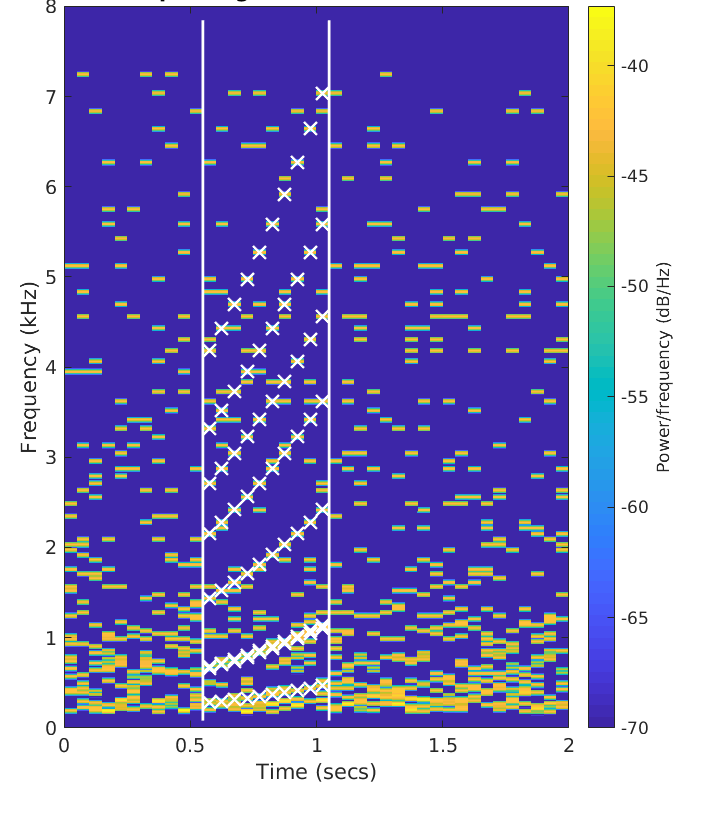
\includegraphics[width=1\linewidth]{sfg_stimulus.png}
		\captionof{figure}{\color{Green} Spectrogram of an example SFG stimulus. The x-axis represents the time the y axis denotes the frequency of the tones and the tone intensity presented by the heatmap (scale shown on the right). The Figure consists of temporally coherent tones that are highlighted with x symbols.}
		\label{fig:stimulus}
	\end{center}
\end{wrapfigure}

\textbf{Participants}:Three groups: Young (N=21, mean age=21.2 yrs), Elderly with normal hearing (N=13, mean age=67.3 yrs), Hearing impaired elderly (N=16, 68.7 yrs)\\
\textbf{Stimuli}: SFG stimuli with or without a figure (see Fig. \ref{fig:stimulus})\\
\textbf{Pre-tests}: An audiometry examination and a digit span test was administered to evaluate hearing and general frontal functionality.\\
\textbf{Stimulus calibration}: Stimuli parameters were adjusted for each participant so that they can all perform the task at the same level of accuracy. The number of consistently rising sound streams (hereinafter: figure coherence) was set for each participant using an adaptive staircase method to values for reaching 60\% and 80\% figure detection accuracy (hereinafter: low SNR and high SNR conditions).

\textbf{Task}: Participants listened to a series of randomly alternating high and low SNR SFG stimuli, each of which either did or did not contain a figure. They needed to decide whether a figure was present. \\
\textbf{Recorded data}: Behavioral measures (accuracy, reaction time) + EEG
\section*{Behavioral results}

	 \textbf{Stimulus calibration successfully compensated for individual performance differences.} The SNR for the high SNR condition was reliably higher than the SNR for the low SNR condition. Consequently, while we found significantly higher Dprime,  lower  R in the high relative to the low SNR condition, there was no evident difference between groups in Dprime, FA or RT. 
	
	 \textbf{Hearing impairment has an effect on FGS ability} The identified SNRs for the HI group were significantly higher than the SNRs for either young and healthy elderly subjects. Similarly, while the noise level was comparable across groups, a more coherent tone composing a coherent object was needed for the hearing impaired group to reach the same performance level as young and healthy older adults.	
	 
	 \begin{center}\vspace{0cm}
	 	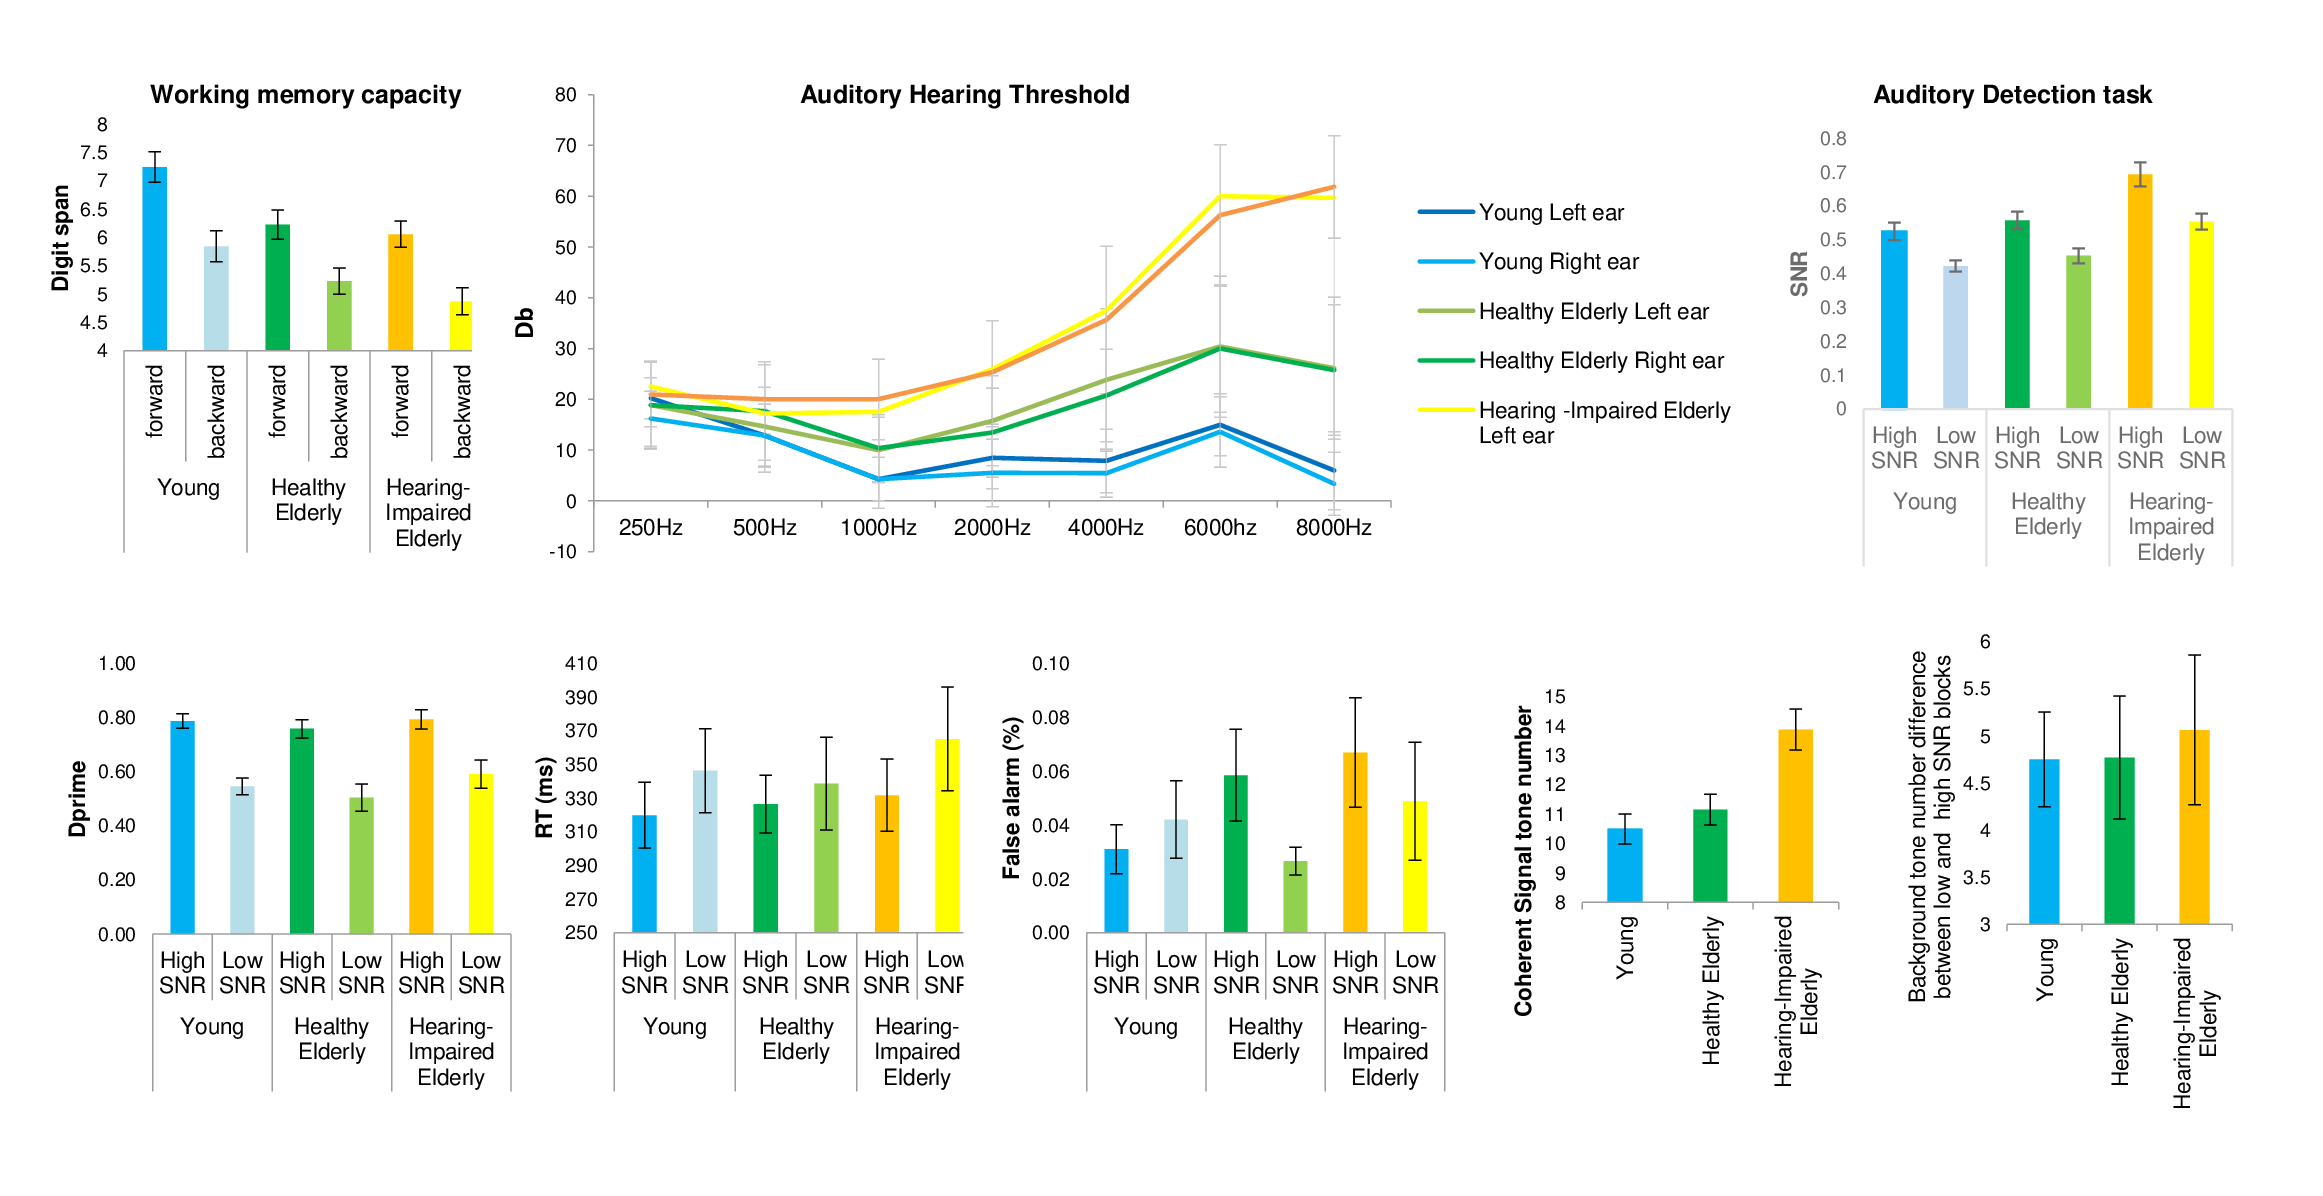
\includegraphics[width=0.95\linewidth]{Fig_behav.png}
	 	\captionof{figure}{\color{Green} Behavioral results}
	 \end{center}\vspace{0cm}
 
 %\vfill\null
 %\columnbreak
 
 \section*{EEG results}
	
	 \textbf{ORN amplitude showed an effect of SNR but no effect of aging or hearing impairment.} The main effect of SNR was found significant due to a higher ORN in case of high SNR trials compared to low SNR trials.
	
	 \textbf{P600 amplitude showed an effect of age but no effect or SNR or hearing impairment.}
	 Post hoc analysis confirmed that age (but not hearing impairment) had a significant effect on the P600 response which was stronger in case of young subjects but did not differ between elderly subjects with normal hearing and hearing impairment.
	
	\textbf{According to source localization, the ORN was elicited in the left Heschl's gyrus, STG, IFG, MFG, MTG, SMG while the P600 component was strongest in the anterior and posterior cingular cortex and posterior brain regions (lingual and pericalcarine gyri)}.

\begin{center}\vspace{0cm}
	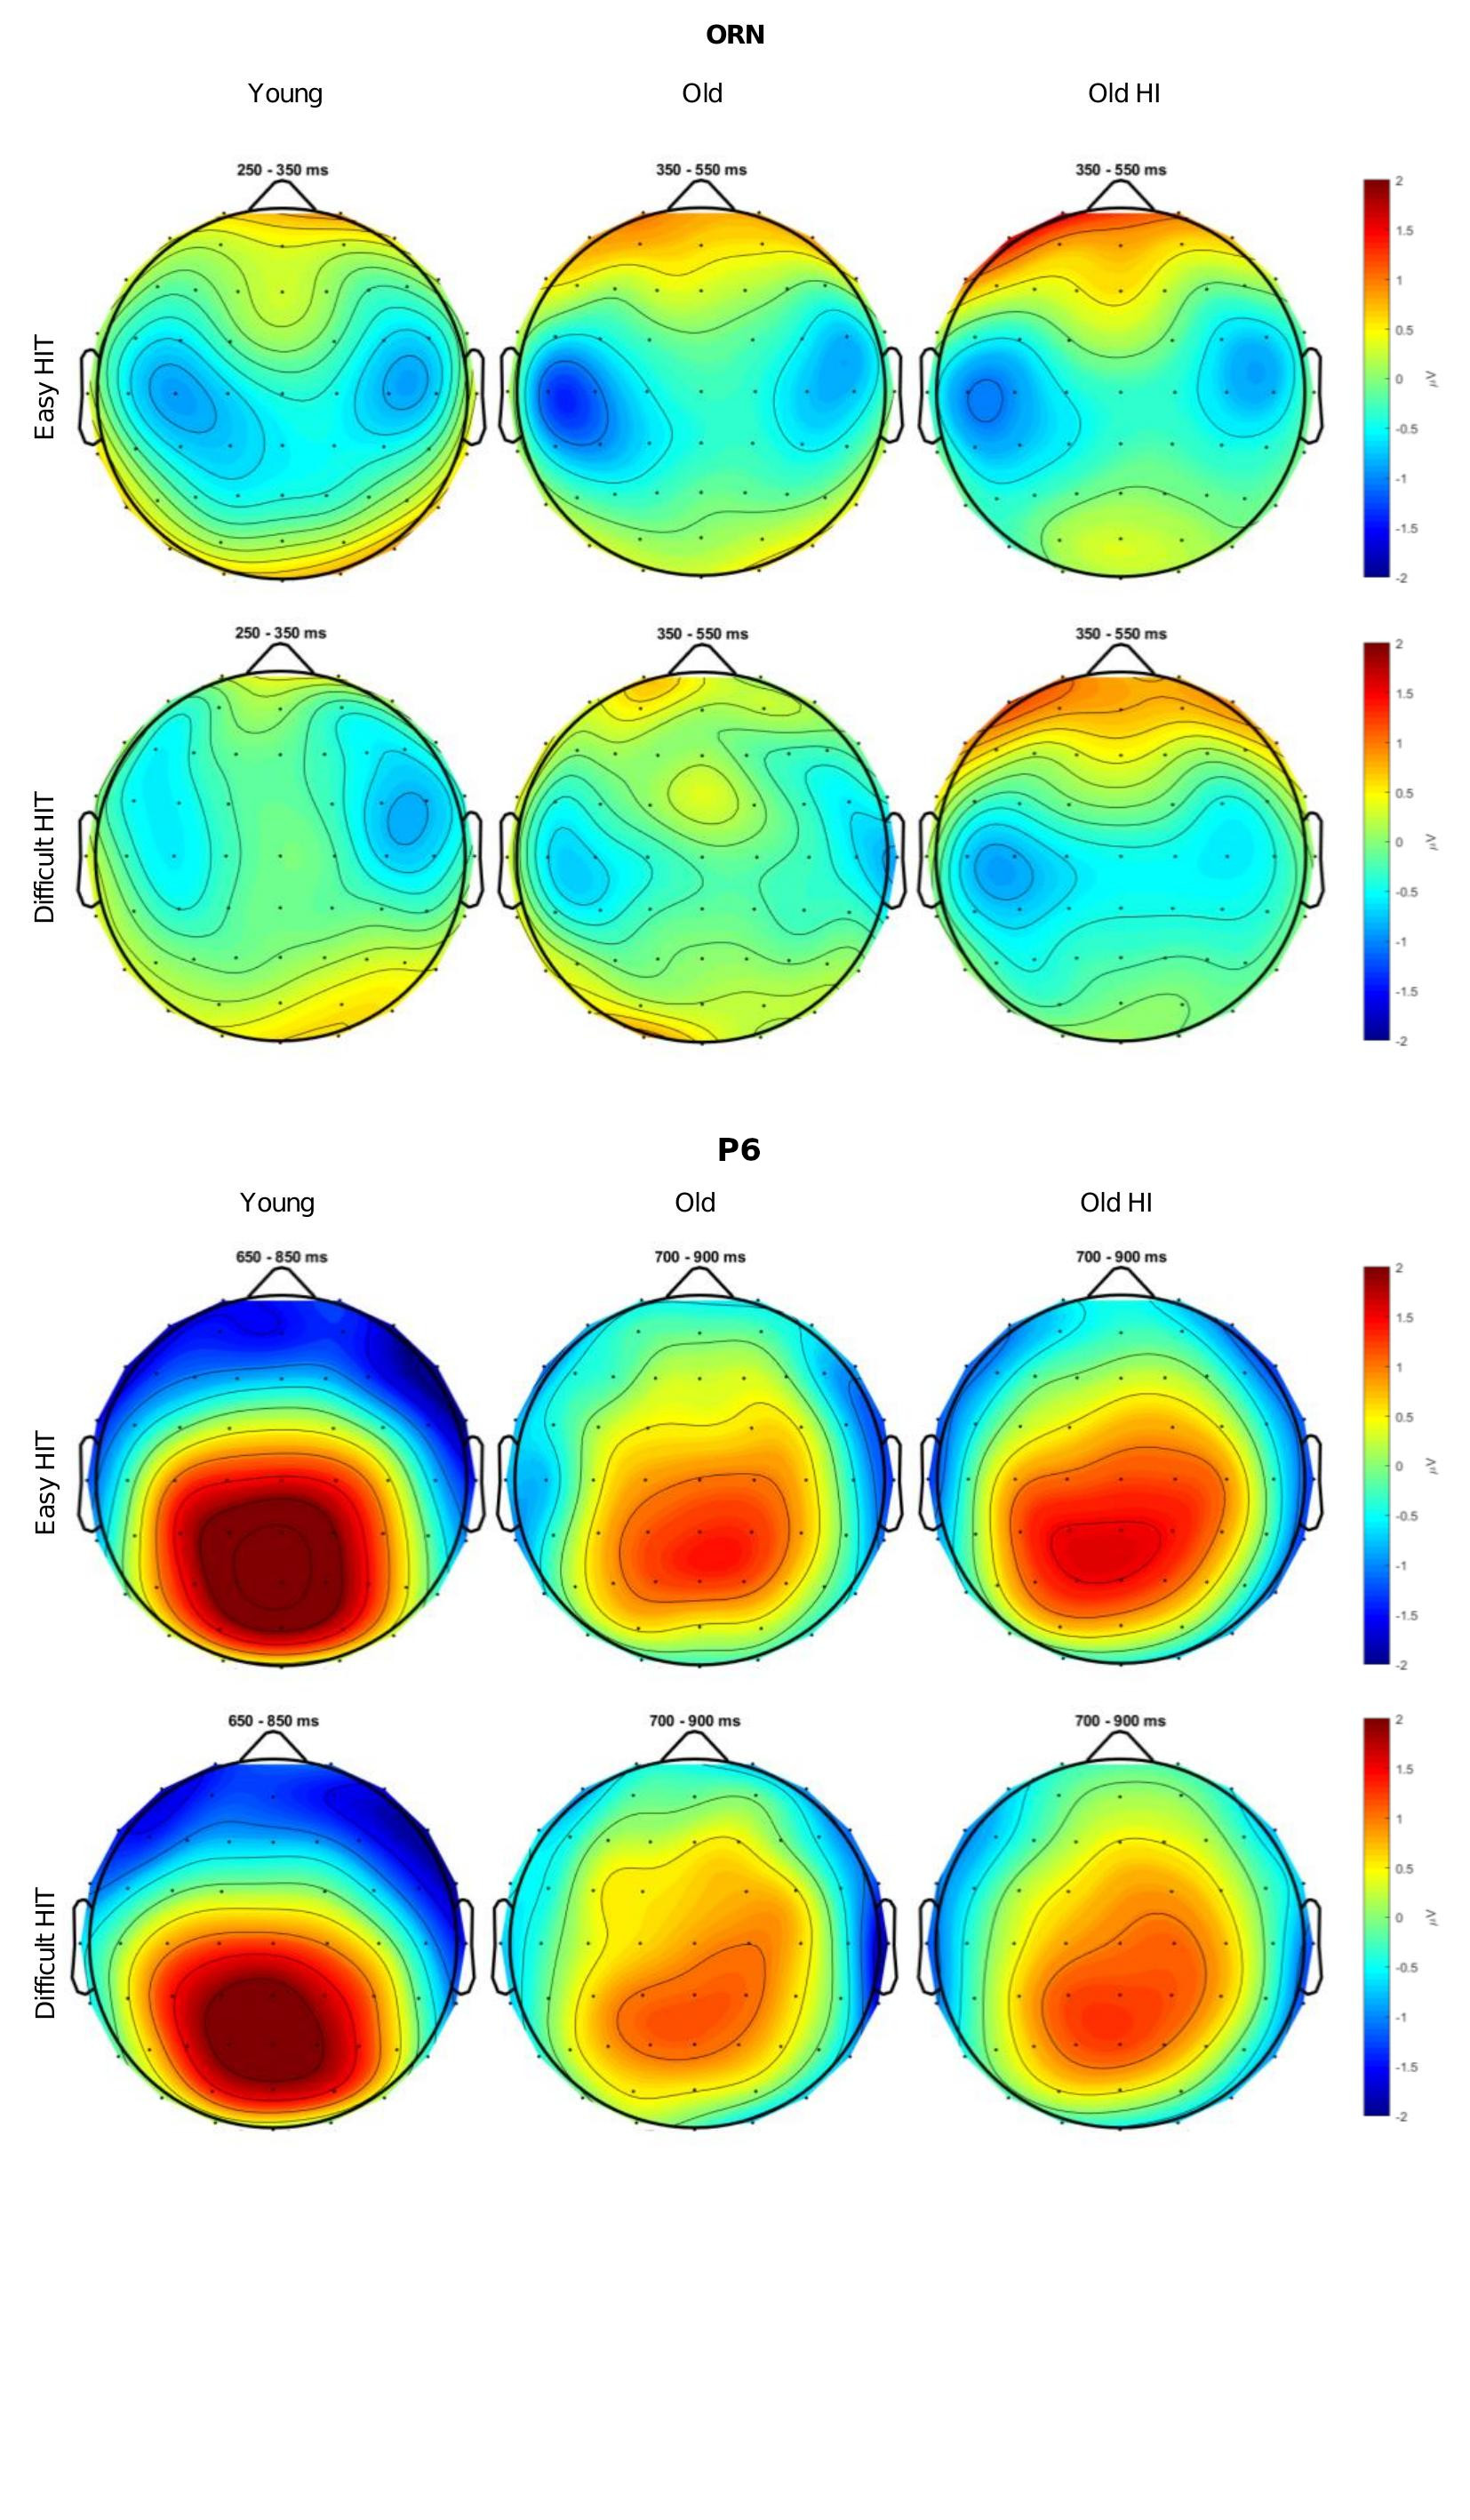
\includegraphics[width=0.35\linewidth]{ORN_P4_4x3.jpg}
	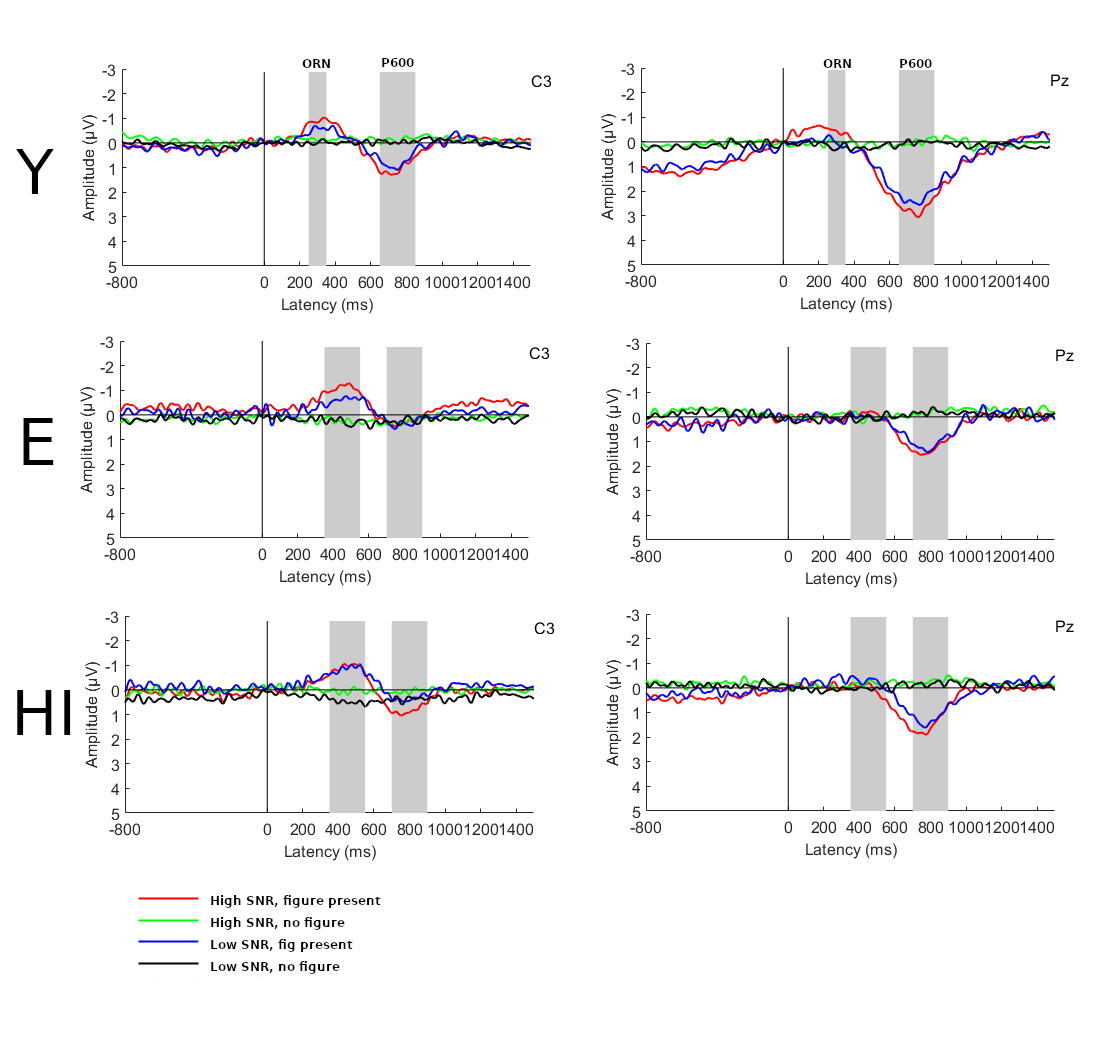
\includegraphics[width=0.6\linewidth]{erps2_legend}
	\captionof{figure}{\color{Green} ORN and P600 event-related potentials (respective time windows marked in grey) on the C3 and Pz electrodes for each group: Y = young, E = elderly with normal hearing, HI = hearing impaired elderly}
\end{center}\vspace{0cm}

%----------------------------------------------------------------------------------------
%	CONCLUSIONS
%----------------------------------------------------------------------------------------

\section*{Conclusions}

The preliminary data from our study that we report here delivers further evidence to the hypothesis that the aging related impairment of auditory object detection in noise is partially accounted for by alterations of brain functionality that are independent of hearing impairment and can also be observed when hearing thresholds are within the normal range. Furthermore, ERP results suggest that age related impairments in listening under noisy conditions mainly affect the later stages of auditory processing while early, low-level object detection mechanisms are intact. Functional connectivity analysis will complement our current findings with further data that might prove informative with regards to the exact neural processes involved. Given the high level of neural plasticity which is still present in the aging brain despite all the anatomical and functional changes \autocite{Grady2012}, gathering information about the impaired neural processes which are independent of the state of the auditory organs themselves opens up the future possibility of developing a treatment method that can significantly improve the everyday life of the elderly by training the affected neural pathways, thereby improving not only their listening skills, but as a consequence of that, improving their feeling of safety and reducing their social isolation which further contribute even to reducing the risk of dementia \autocite{Slade2020}.

%----------------------------------------------------------------------------------------
%	FORTHCOMING RESEARCH
%----------------------------------------------------------------------------------------

\section*{Forthcoming Research}

Our forthcoming study will address the question of whether figure-ground segregation training can improve the ability to listen in a noisy environment in aging.

 %----------------------------------------------------------------------------------------
%	REFERENCES
%----------------------------------------------------------------------------------------
\vspace{100pt}
\subsection*{References}
\AtNextBibliography{\tiny}
\printbibliography[heading=none]

%----------------------------------------------------------------------------------------
%	ACKNOWLEDGEMENTS
%----------------------------------------------------------------------------------------

\subsection*{Acknowledgements}
\tiny
This research project has been supported by grant nr. 123790 of the Hungarian Scientific Research Fund (OTKA) and a Bolyai Grant received by the Sound and Speech Perception Research Group of the Institute of Cognitive Neuroscience and Psychology at the Research Centre for Natural Sciences (Principal investigator: Brigitta Tóth).

%----------------------------------------------------------------------------------------

\end{multicols}
\end{document}